\documentclass{bioinfo}
\copyrightyear{2012}
\pubyear{2012}

\begin{document}
\firstpage{1}

\title[Scythe]{Scythe: A tool for removing 3'-end adapter contaminants using Bayesian classification}
\author[Buffalo \textit{et~al}]{Vince Buffalo\,\footnote{to whom correspondence should be addressed}, Joseph Fass\, and Dawei Lin}
\address{Bioinformatics Core, UC Davis Genome Center}

\history{Received on XXXXX; revised on XXXXX; accepted on XXXXX}

\editor{Associate Editor: XXXXXXX}

\maketitle

\begin{abstract}

\section{Motivation:}
Illumina's short read sequencing technology uses known adapter
sequences that can contaminate the 3'-ends of reads when individual
sample fragments are shorter than the read length. Unfortunately, the
3'-ends of these reads are enriched with low quality bases that are
more likely to be called incorrectly, which makes identifying and
removing 3'-end contaminants difficult. However, removal of
contaminating sequence is a critical step in most bioinformatics
pipelines.


\section{Results:} 
We have written Scythe - a novel 3'-end adapter trimmer based on
Bayesian classification that considers both sequence and base
qualities. In our tests, Scythe outperforms other adapter removal
tools across a wide range of contamination rates, and is more robust
to parameter settings than other tools.


\section{Availability:}
Scythe is freely available under the MIT license at
\href{http://github.com/vsbuffalo/scythe}{http://github.com/vsbuffalo/scythe}.


\section{Contact:} \href{mailto:vsbuffalo@gmail.com}{vsbuffalo@gmail.com}
\end{abstract}


\section{Introduction}
Scythe embraces the Unix Philosophy of ``programs that do one thing
well'' (\citealp{raymond2003}), and focuses on recognition and
trimming of Illumina adapter contamination. Illumina's
second-generation sequencing technology (MiSeq, GA series, HiSeq)
often results in reads that have a known, largely unvarying adapter
sequence that starts at variable (but largely 3'-biased) positions in
reads. Bases at the 3'-end are also more difficult to call, and
accordingly have low base qualities and high substitution error
rates. Importantly, though, the 3'-end quality deterioration is not
uniform across all reads (see Fig. 1 in Supplementary Materials).

Low quality 3'-end bases are commonly trimmed as a first step, however
this discards some evidence, albeit noisy, for adapter
sequences. Scythe is meant to be run before quality trimming is
performed, and uses a Bayesian classification scheme that
differentially weights mismatches between the adapter sequence and
bases in a read according to their particular base quality.

We tested Scythe using a combination of real and simulated data, along
with two other 3'-end adapter trimming tools: Btrim (ref) and Cutadapt
(ref).

% A common step in read quality improvement procedures is to remove
% these low-quality 3'-end sequences from reads. This is thought to
% increase mapping rates and improve assembly quality. However doing
% quality-based 3'-end trimming before contaminant removal would remove
% sequence that could be used (despite being unreliable) to identify the
% contaminants more accurately. Scythe takes the approach that it is
% better to use full information, even if it's unreliable. How
% unreliable a base is is indicated by the FASTQ quality score, which
% can be incorporated into Scythe's classification procedure.

% Fixed-number of mismatch approaches have the disadvantage that they
% do not differentially weight a mismatch on a low-quality base from a
% mismatch on a high-quality base. Futhermore, the fixed-number could
% easily be exhausted in a run of bad bases (which are quite common in
% the 3'-end), even though every good-quality base perfectly matches the
% contaminant sequence.


\begin{methods}
\section{String Matching in Scythe}

Scythe employs a simple, string matching heuristic to find a best
match for a given contaminant sequence within a given read. Scythe
scores ungapped alignments of the contaminant sequence against the
read sequence, from a minimum overlap at the 3'-end (by default, 5 bp)
to full overlap with right justification of the contaminant within the
read. Each of these alignments is scored using a scheme of $1$ for a
match, $-1$ for a mismatch. The top scoring alignment is then passed
to the probabilistic classification procedure, described below. The
time complexity of Scythe's matching algorithm for a single adapter of
length $l_a$ is $O(l_a^2 R)$ for a FASTQ file with $R$ entries.


\section{Bayesian Classification of Top-Scoring Matches}

Considering the highest-scoring alignment of a contaminant sequence to
a read, there are two mutually exclusive and exhaustive events: (1)
there is a contaminant at the specified position, or (2) there is no
contaminant at that position. A likelihood for each of these events,
given probabilities of each base being called correctly (derived from
the base qualities) and which bases mismatch the contaminant sequence,
can be calculated.

These likelihood functions assume models of error for each event. If
the top-scoring match is contaminant-derived (event $C$), the
likelihood $P(S | C)$ (where $S$ is the sequence match data) is:

$$ P(S | C) = \prod_{i=1}^{l_t} q_i^{m_i} \cdot (1-q_i)^{1 - m_i} $$

Where $m_i \in \{0, 1\}$ indicating whether the $i$ base is a mismatch
or match (respectively) and $q_i$ is the probability the $i$ base is
called correctly (from its base quality). $l_t$ is the length of the
top-scoring match. On the other hand, if the top-scoring match is not
contaminant-derived (event $C'$), it is assumed that the match
occurred by chance, giving the likelihood function:

$$ P(S | C') = \prod_{i=1}^{l_t} \left(\frac{1}{4}\right)^{m_i} \cdot \left(\frac{3}{4}\right)^{1 - m_i} $$

These likelihoods can then be combined using Bayes' Thereom to give
the probability of contamination given the top-scoring match:

$$ P(C|S) = \frac{P(C) P(S|C)}{P(S)} $$

Since these are mutually exclusive and exhaustive events, the
\emph{maximum a posteriori} rule can be used to classify a top-scoring
alignment as due to contamination (if $P(C|S) > P(C'|S)$) or chance (if
$P(C'|S) > P(C|S)$).

Required in this Bayesian formulation is the prior of contamination,
$P(C)$. This can be estimated by inspection of the sequences
(i.e. counting perfect matches to a substring of the adapter
sequence), though in practice Scythe's performance does not depend on
an accurate estimate. More information on specifying the prior is in
Supplementary Materials.

\section{Results}
\begin{centering}
\begin{figure*}[!tpb]
\includegraphics[angle=-90]{graphics/roc-and-incorrect-trimmed.eps}
\caption{ROC curve showing Scythe's higher rate of true positives for
  a given false positive rate and a bar chart indicating Scythe's
  fewer incorrectly trimmed reads.}\label{fig:02}
\end{figure*}
\end{centering}

Scythe was tested against two similar program: Btrim
(\citealp{pmid21651976}) and Cutadapt (\citealp{EJ200}). Both Btrim
and Cutadapt can handle insertions/deletions, but these are rare in
Illumina sequences. Whereas Btrim and Cutadapt also perform quality
trimming, Scythe intentionally limits its scope to adapter trimming.

To test these tools, random reads were generated and contaminated at
fixed contamination rates of 40\% and 70\%, and paired to base quality
profiles from an Illumina HiSeq run, followed by mutation of each base
at the rate designated by their base quality (i.e. a base with a
quality score of 30 had a 1 in 1000 chance of being changed to a
different, random base). For each contamination rate, ten replicate
FASTQ files of 10,000 sequences each were generated, to ensure that
contaminated and non-contaminated reads were well dispersed across
different base quality profiles.

Each program was run with varying parameters to see how true positive
and false positive rates change. Btrim uses a fixed number of
mismatches, so integer values from 0 to 10 were used. Cutadapt uses an
error rate for a matched sequence, which was varied from 0 to 0.95 in
0.05 increments. Scythe uses the same values as Cutadapt, for the
prior. Each program was run with all other options off to ensure a
fair comparison of 3'-end contaminant removal.

While Cutadapt and Scythe only trim reads, Btrim occasionally removes
a read entirely from the sample. For comparison purposes, we count
this as trimming the entire length of a read. We compared the length
of the original simulated read to the trimmed read for all programs,
parameters, replicates, and contamination rates, in order to calculate
true positive and false positive rates. We also counted how many times
Btrim, Cutadapt, and Scythe incorrectly trimmed a read, e.g. whether
the trimmed length was not equal to the contaminated length for reads
that were contaminated.

All three tools performed almost almost identically at the 40\% and
70\% contamination rates (Fig. \ref{fig:02}a). Scythe outperformed
Btrim and Cutadapt in terms of true positive rates for a variety of
false positive rates across a wide range of parameters
(Fig. \ref{fig:02}). In addition, Scythe's performance (TP/FP rates)
was relatively stable across a wide range of priors - most notably
between ~0.45 and 0.95, whereas small parameter changes had large
effects on the TP/FP rates for Cutadapt and Btrim. Scythe also has
fewer incorrectly trimmed reads across a variety of parameters
compared to Btrim and Cutadapt (Fig. \ref{fig:02}b).

\end{methods}


\section{Conclusion}

When compared to Btrim and Cutadapt, Scythe outperforms both in terms
of the True Positive (TP) rate across a large range of input
parameters, and Scythe would not generate results with a False
Positive (FP) rate above ~0.4 in the data tested. Scythe's 'prior'
parameter can be set through straightforward inspection of the reads
(for perfect matches), and is more weakly correlated with the FP rate,
meaning inaccurate settings will not suddenly cause poor performance.

In Scythe, we have implemented an approach to 3'-end contaminant
trimming that is novel in two respects: (1) consideration of
base-level qualities and (2) the use of a Bayesian model rather than a
simple fixed-number of mismatches or fixed-error approach. We believe
that this approach can improve contaminant removal in many pipelines
and applications.


\section*{Acknowledgement}
Monica Britton and Nikhil Joshi for helpful feedback about bugs in
Scythe. Xiran Dong was very helpful in early testing of Scythe against
other trimmers.

%\paragraph{Funding\textcolon} None.


\bibliographystyle{natbib}
% \bibliographystyle{achemnat}
% \bibliographystyle{plainnat}
% \bibliographystyle{abbrv}
% \bibliographystyle{bioinformatics}
\nocite{qrqc}
\nocite{ShortRead}
\nocite{Biostrings}
\nocite{ggplot2}

\bibliography{references}


\end{document}
